% !TEX encoding = UTF-8
% !TEX TS-program = pdflatex
% !TEX root = ../tesi.tex
% !TEX spellcheck = it-IT

%**************************************************************
\chapter{Analisi dei requisiti}
\label{cap:analisi-requisiti}
%**************************************************************

Sin dalla sua concezione, la piattaforma Plot è stata pensata come un prodotto unico e fatto su misura per il cliente. Questo ha impedito la definizione di una struttura di base sulla quale innestare eventuali cambiamenti. \\
La prima attività del progetto è stata dunque la consultazione dello schema del database e del codice relativo al CMS di Plot 1.0. Successivamente sono state intervistate le persone coinvolte nello sviluppo di Plot 1.0: developer, responsabili dei contenuti ed utilizzatori del CMS in modo da capire cosa non li soddisfacesse nella struttura attuale e cosa potesse essere fatto per migliorarla.
Da queste interviste sono stati sintetizzati i requisiti che il database ed il CMS avrebbero dovuto avere. Tali requisiti sono stati fondamentali per la successiva progettazione ma possono risultare utili anche all'azienda per valutare in modo più razionale limiti e possibilità della piattaforma.

\section{Il database}
\subsection{Descrizione dei requisiti}
Un \textbf{consumer} è un concetto astratto che rappresenta un generico utilizzatore della piattaforma Plot, esso è caratterizzato da nome, cognome, email e password.
Un consumer può concretizzarsi nel concetto di admin o user. \\
Un \textbf{admin} rappresenta un amministratore del CMS, ha quindi l'autorizzazione di accedere al CMS ma non può accedere alla parte di gioco. \\ 
Uno \textbf{user} rappresenta un utente del gioco e può quindi accedere alla parte di gioco ma non al CMS. \\
Solitamente i consumer si autenticano presso la piattaforma tramite email e password ma può capitare che gli user utilizzino un servizio di autenticazione esterno tramite \textit{token}.
\\ \\
Un \textbf{invitation} rappresenta un invito che può essere spedito o ricevuto da uno user durante la fase di inviti. Un invitation è caratterizzato dal mittente e dal destinatario, che dovranno essere entrambi user.
\\ \\
Terminata la fase di inviti, ogni user appartiene ad un \textbf{team} caratterizzato da un nome e da un'immagine rappresentativa dello stesso. I team vengono creati a priori e sono associati agli user solo al termine della fase di inviti. 
\\ \\
Qualsiasi richiesta HTTP effettuata da uno user nel front end di gioco genera un \textbf{log} contenente:
\begin{itemize}
	\item Un riferimento allo user che ha effettuato la richiesta;
	\item Indirizzo IP del dispositivo che ha effettuato la richiesta;
	\item Il metodo HTTP utilizzato per la richiesta;
	\item L'URL al quale è stata inoltrata la richiesta;
	\item Lo user agent che ha effettuato la richiesta;
	\item Eventuali dati aggiuntivi trasportati dalla richiesta.
\end{itemize}  

Un \textbf{language} rappresenta una lingua parlata ed è caratterizzato da un nome (es. Italiano) e da un codice identificativo (es. it). \\
Una \textbf{translation} rappresenta una traduzione disponibile per un certo contenuto in un particolare language.
Ogni user può indicare il proprio language preferito e questa informazione può essere utilizzata per fornire i contenuti di gioco localizzati in base allo user.
\\ \\
Uno user può appartenere ad una \textbf{category}, il significato della category non è fissato a priori ma può essere istanziato in base alle necessità del progetto e del cliente che lo richiede. Il concetto di category è quindi astratto e viene utilizzato per partizionare gli user sulla base di una o più caratteristiche.  
Ad esempio, gli user possono essere categorizzati per regione di appartenenza o per posizione lavorativa. Una category ha un nome che la identifica. \\
Per questo progetto vengono istanziate le due category più usate nei Plot passati: region e business role.\\
Una \textbf{region} rappresenta l'area del mondo alla quale appartiene un certo user ed è caratterizzata da una timezone. Una \textbf{timezone} identifica un particolare fuso orario ed è caratterizzata dal nome (es. Central European Time), dal codice identificativo della timezone (es. CET) e dall’offset rispetto allo UTC (es. +1).
Una region può quindi rappresentare un insieme di stati, un singolo stato o una porzione di esso, questo dipende dallo specifica istanza di Plot.\\
Un \textbf{business role} rappresenta il ruolo dello user all'interno dell'azienda o, più in generale, l'area lavorativa alla quale esso afferisce.
\\ \\
Un Plot è composto da una o più \textbf{mission}. Ogni mission è caratterizzata da un nome, un'immagine rappresentativa, una data d'inizio e una data di fine, oltre la quale la mission si considera chiusa.
Una mission è composta da più \textbf{post}. Ogni post prevede un testo ed appartiene ad una delle seguenti tipologie: 
\begin{itemize}
	\item \textbf{Text post};
	\item \textbf{Captcha post}: prevede una domanda indirizzata ai singoli user;
	\item \textbf{Team post}: prevede una domanda indirizzata ai team. 
\end{itemize}

Una \textbf{question} è un concetto astratto che rappresenta una generica domanda, essa prevede un testo che riporta il corpo della domanda stessa. Una question può essere istanziata da una user question o da una team question.\\
Una \textbf{user question} rappresenta una domanda indirizzata ai singoli user. Le user question sono caratterizzate dalle category alle quali sono rivolte. Se il concetto di category è utilizzato dalla particolare istanza di Plot, è possibile assegnare domande diverse a user appartenenti a diverse category. Viceversa, se il concetto di category non è utilizzato, ogni domanda può potenzialmente essere assegnata ad ogni user.
Una user question è visibile alla pubblicazione del captcha post al quale appartiene.\\
Una \textbf{team question} rappresenta una domanda indirizzata ai team. Le team question prevedono un tempo limite entro il quale devono ricevere risposta. Qualsiasi componente del team può fornire una o più risposte ad una specifica domanda.
Una team question non è immediatamente visibile alla pubblicazione del team post al quale appartiene, per svelarla è necessario che un componente del team dichiari di volerla visualizzare, a quel punto la domanda è visualizzabile da tutti i membri del team. Nel momento in cui uno user decide di svelare una domanda, viene inizializzato un timer che decreta il tempo impiegato dal team per fornire una risposta corretta. Una funzione del tempo impiegato andrà a decretare il punteggio totalizzato dal team nella specifica mission. Il punteggio totale di un team è dato dalla somma dei punteggi totalizzati dal team nelle varie mission e, sulla base di questo, viene stilata la classifica dei team.
\\ \\
Una \textbf{correct answer} rappresenta una risposta corretta prevista per una specifica question, ogni question deve prevedere almeno una risposta corretta.
Ogni user può fornire più risposte alle question proposte, una risposta ad una question è considerata corretta se e solo se il suo contenuto compare tra le correct answer previste per la specifica question.
\\ \\
Uno user può visualizzare un post più volte e, lo stesso post, può essere visualizzato da user diversi.
\\ \\
Un admin può decidere se mostrare (o mantenere nascosta) agli user una mission o un post.
\\ \\
Deve essere possibile fornire una translation per i contenuti testuali di mission, post, question ed in generale tutti gli elementi di gioco con i quali entra in contatto lo user.

\subsection{L'integrazione con Eloquent}
Per poter sfruttare appieno le potenzialità di Eloquent, l'ORM fornito con Laravel, è necessario rispettare alcune convenzioni:
\begin{itemize}
	\item Lo schema di ogni tabella appartenente al database deve prevedere le colonne \verb!created_at! e \verb!updated_at!. Il valore relativo a queste colonne viene automaticamente inserito dall'ORM ogniqualvolta venga creato o modificato un record;
	\item Lo schema di ogni tabella appartenente al database deve prevedere una colonna relativa alla primary key e tale colonna deve chiamarsi \verb!id!;
	\item I nomi di tabelle ed attributi devono essere in minuscolo e seguire la convenzione snake case;
	\item I nomi delle tabelle devono essere pensati al plurale. Ad esempio, la tabella contenente i captcha post dovrà essere chiamata \verb!captcha_posts!;
		\item Gli attributi che fungono da foreign key devono essere nominati posponendo "`id"` al nome singolare della tabella alla quale si riferiscono. Ad esempio, una foreign key che si riferisca alla tabella users dovrà essere chiamata \verb!user_id!.
\end{itemize}

\section{Il CMS}

\subsection{Casi d'uso}

Per lo studio dei casi di utilizzo del prodotto sono stati creati dei diagrammi.
I diagrammi dei casi d'uso (in inglese \emph{Use Case Diagram}) sono diagrammi di tipo \gls{uml} dedicati alla descrizione delle funzioni o servizi offerti da un sistema, così come sono percepiti e utilizzati dagli attori che interagiscono col sistema stesso.
Essendo il progetto finalizzato alla creazione di un tool per l'automazione di un processo, le interazioni da parte dell'utilizzatore devono essere ovviamente ridotte allo stretto necessario. Per questo motivo i diagrammi d'uso risultano semplici e in numero ridotto.

\begin{figure}[!h] 
    \centering 
    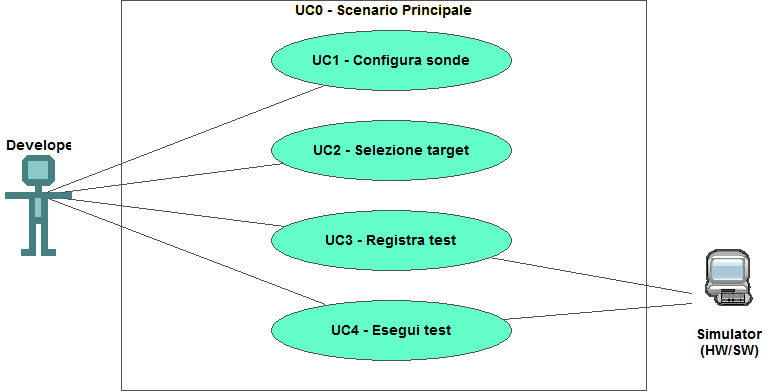
\includegraphics[width=0.9\columnwidth]{usecase/scenario-principale} 
    \caption{Use Case - UC0: Scenario principale}
\end{figure}

\begin{usecase}{0}{Scenario principale}
\usecaseactors{Sviluppatore applicativi}
\usecasepre{Lo sviluppatore è entrato nel plug-in di simulazione all'interno dell'IDE}
\usecasedesc{La finestra di simulazione mette a disposizione i comandi per configurare, registrare o eseguire un test}
\usecasepost{Il sistema è pronto per permettere una nuova interazione}
\label{uc:scenario-principale}
\end{usecase}

\section{Tracciamento dei requisiti}

Da un'attenta analisi dei requisiti e degli use case effettuata sul progetto è stata stilata la tabella che traccia i requisiti in rapporto agli use case.\\
Sono stati individuati diversi tipi di requisiti e si è quindi fatto utilizzo di un codice identificativo per distinguerli.\\
Il codice dei requisiti è così strutturato R(F/Q/V)(N/D/O) dove:
\begin{enumerate}
	\item[R =] requisito
    \item[F =] funzionale
    \item[Q =] qualitativo
    \item[V =] di vincolo
    \item[N =] obbligatorio (necessario)
    \item[D =] desiderabile
    \item[Z =] opzionale
\end{enumerate}
Nelle tabelle \ref{tab:requisiti-funzionali}, \ref{tab:requisiti-qualitativi} e \ref{tab:requisiti-vincolo} sono riassunti i requisiti e il loro tracciamento con gli use case delineati in fase di analisi.

\newpage

\begin{table}%
\caption{Tabella del tracciamento dei requisti funzionali}
\label{tab:requisiti-funzionali}
\begin{tabularx}{\textwidth}{lXl}
\hline\hline
\textbf{Requisito} & \textbf{Descrizione} & \textbf{Use Case}\\
\hline
RFN-1     & L'interfaccia permette di configurare il tipo di sonde del test & UC1 \\
\hline
\end{tabularx}
\end{table}%

\begin{table}%
\caption{Tabella del tracciamento dei requisiti qualitativi}
\label{tab:requisiti-qualitativi}
\begin{tabularx}{\textwidth}{lXl}
\hline\hline
\textbf{Requisito} & \textbf{Descrizione} & \textbf{Use Case}\\
\hline
RQD-1    & Le prestazioni del simulatore hardware deve garantire la giusta esecuzione dei test e non la generazione di falsi negativi & - \\
\hline
\end{tabularx}
\end{table}%

\begin{table}%
\caption{Tabella del tracciamento dei requisiti di vincolo}
\label{tab:requisiti-vincolo}
\begin{tabularx}{\textwidth}{lXl}
\hline\hline
\textbf{Requisito} & \textbf{Descrizione} & \textbf{Use Case}\\
\hline
RVO-1    & La libreria per l'esecuzione dei test automatici deve essere riutilizzabile & - \\
\hline
\end{tabularx}
\end{table}%